\chapter{Een compositie en aggregatie.}
\label{ch:hfstCompAgg}
Bij deze opdracht zal een aggregatie en compositie in C++ geïmplementeerd worden. Met behulp van de DDD debugger worden objecten en hun onderlinge verbindingen zichtbaar gemaakt. Hiervan zullen verschillende screenshots gemaakt moeten worden die opgenomen  moeten worden in je portfolio. De portfolio moet aan het einde van de week geüpload worden op Brightspace. Tijdens het aftekenen moeten de screenshots zichtbaar zijn.
Op de screenshots zal je \textbf{eigen} \textcolor{BrickRed}{\textbf{naam}} en \textcolor{BrickRed}{\textbf{studienummer}} moeten staan.

De opdracht bestaat uit een speciaal type LED, de LogLed. De LogLed heeft als extra een stopwatch,en een Tijdsduur. De klasse wordt weergegeven in figuur \ref{fig:logled}.
    \begin{figure}[h!]
	\captionsetup{justification=centering}
	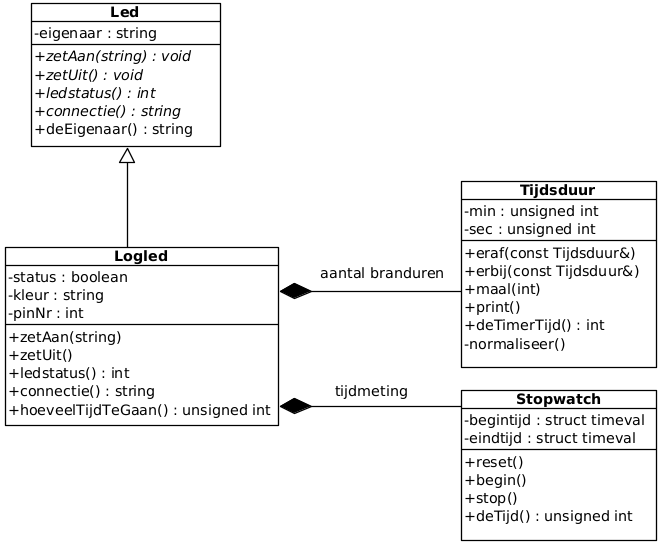
\includegraphics[width=0.9 \linewidth]{figuren/logled}      %ledPlatform}
\centering
\caption{De logled met timer en stopwatch.}
\label{fig:logled}
\end{figure} 
De logled is speciaal ontwikkelt om ervoor te zorgen dat een LED maar een maximum aan uren aan kan. daarna moet een nieuwe logled gekocht worden. 
\begin{itemize}
	\item Met het tijdsduur wordt bijgehouden hoeveel minuten de logled nog aan mag. 
	\item Met de stopwatch wordt elke keer gecheckt hoelang de logled voor dat moment aan is.
	\item De Led kan hergebruikt worden uit de vorige opgave, De stopwatch krijg je cadeau en is te downloaden van github. \\De klasse Logled en Tijdsduur moet je zelf maken.
\end{itemize}

\section{De klasse Tijdsduur.}

We willen een ADT (Abstract Data Type) , ook wel zelfgedefinieerd datatype genoemd, maken waarin een tijdsduur in minuten en seconden kan worden opgeslagen. De totale tijd in seconden kan ook worden opgevraagd. 
\begin{figure}[h!]
	\captionsetup{justification=centering}
	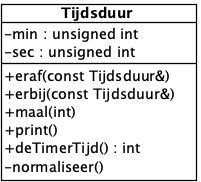
\includegraphics[width=0.28 \linewidth]{figuren/tijdsduur}
	\centering
	\caption{weergave van de klasse Tijdsduur. }
	\label{fig:tijdsduurKlas}
\end{figure}
We noemen dit zelf gedefinieerde datatype \texttt{Tijdsduur}. Figuur \ref{fig:tijdsduurKlas} geeft de klasse weer van Tijdsduur.
Het ADT \texttt{Tijdsduur} kan in C++ als volgt gedeclareerd worden in de header file (tijdsduur.h):

\begin{lstlisting}[caption= de headerfile van de klasse \texttt{Tijdsduur},label={lst:tijdsdHeader},numbers=none]		
	#ifndef TIJDSDUUR_H
	#define TIJDSDUUR_H
	
	// De declaratie van de ADT Tijdsduur:
	class Tijdsduur {
		public:
		//...
		void eraf(Tijdsduur t);
		//...
		
		private:
		int sec;
		//...
	};
	#endif // TIJDSDUUR_H
\end{lstlisting}

De implementatie (\texttt{tijdsduur.cpp}) ziet er tot nu toe als volgt uit:
\begin{lstlisting}[caption= de implementatiefile van de klasse \texttt{Tijdsduur},label={lst:tijdsdImpl},numbers=none]
	#include <iostream>
	#include "tijdsduur.h"
	#include <iomanip>
	using namespace std;
	
	// De definities van de memberfunctie van de ADT Tijdsduur, oftewel: de implementatie van de ADT Tijdsduur:
	void Tijdsduur::eraf(Tijdsduur t) {
		sec-=t.sec;
		//...
	}
\end{lstlisting}

Het hoofdprogramma (\texttt{opg13.cpp}) ziet er als volgt uit:

\begin{lstlisting}[caption= de implementatiefile van het hoofdprogramma ,label={lst:tijdsdMainprog},numbers=none]
	#include <iostream> // nodig voor cout (schrijven naar scherm)
	#include <iomanip> // nodig voor setw (veldbreedte definieren )
	#include "tijdsduur.h"
	using namespace std;
	
	int main() {
		Tijdsduur t1(3,50); // t1 is 3 minuten en 50 seconden
		cout<<"t1 = "; t1.print(); cout<<endl;
		const Tijdsduur kw(15); // kw is 15 seconden
		cout<<"kw = "; kw.print(); cout<<endl;
		t1.erbij(kw); // Tel kw bij t1 op
		cout<<"t1 = "; t1.print(); cout<<endl;
		Tijdsduur t2(t1); // t2 is een kopie van t1
		t2.eraf(kw); // Trek kw van t2 af
		cout<<"t2 = "; t2.print(); cout<<endl;
		t2.maal(7); // Vermenigvuldig t2 met 7
		cout<<"t2 = "; t2.print(); cout<<endl;
		Tijdsduur t3(3,-122); // t3 is 3 minuten minus 122 seconden
		cout<<"t3 = "; t3.print(); cout<<endl;
		t3.eraf(t2); 
		cout<<"t3 = "; t3.print(); cout<<endl;
		Tijdsduur t4(3,122); // t4 is 3 minuten plus 122 seconden
		cout<<"t4 = "; t4.print(); cout<<endl;
		cout<<"het totaal aantal seconde van t4 = "<<t4.deTimerTijd()<<endl;
		return 0;
	}	
\end{lstlisting}
De uitvoer moet dan zijn:

\begin{tabular}{ l l l }
	t1= & 3 minuten en & 50 seconden \\ 
	kw	=& &15	seconden \\  
	t1	=&	4	minuten en&	5	seconden\\
	t2	=&	3	minuten en	&50	seconden\\
	t2	=&	26	minuten en	&50	seconden\\
	t3	=&			&58	seconden\\
	t3	=&			&0	seconden\\
	t4	=&	5	minuten en	&2	seconden
	
\end{tabular}

\paragraph{Opdracht}
\begin{enumerate}[label=\alph*]
	\item De code van de implementatie van de klasse tijdsduur, zoals hierboven vermeld is, is verre van compleet.
	Download  opg13.zip van Brightspace of clone deze:\\ 
	{\small \texttt{git clone } \verb|--| \texttt{branch logled https://github.com/JohnVi-hhs/oop.git}}
	
	Vul de declaratie en de implementatie van de ADT genaamd  Tijdsduur verder in. Zorg ervoor dat het hoofdprogramma (\texttt{testTijdsduur.cpp}) zonder warnings te compileren is en de gewenste uitvoer produceert. Zoek (indien nodig) inspiratie bij de in de les behandelde \texttt{\textbf{class} Breuk}. Tip: Zorg ervoor dat de opgeslagen seconden altijd \textgreater =0 en \textless 60 zijn.
	\item Voer zelf nog een aantal testen met Tijdsduur uit. B.v het gebruik van de methode\texttt{ int deTimerTijd()}.
	\item Laat de opdracht aftekenen.
\end{enumerate}


\subsection{De klasse Logled}

Zoals uit figuur \ref{fig:logled} blijkt heeft de klasse \textbf{Logled} twee compositie klassen namelijk de Klasse \textbf{Tijdsduur} en \textbf{Stopwatch}.



\begin{comment}

\begin{enumerate}[label= \alph*]
	\item Download de directory met de klassen RockPi en RockPiPin en blink2.cpp van Brightspace of clone deze:\\ 	\textit{git clone~ -~-branch RockOpg21 https://github.com/Johnny63Vi/oopr1.git}
	Het main programma (blink2.cpp) wordt weergegeven in Listing \ref{lst:mainLed}.
	\begin{lstlisting}[caption= de implementatiefile van het hoofdprogramma om de led en platform te testen ,label={lst:mainLed}]
#define TIMELEDON 1000000
#define TIMELEDOFF 500000

int main (void)
{
	cout<<"hoi opgave "<<endl;
	
	/* 
	De rock pi wordt gebruikt om de pinnen aan te sturen.
	*/
	
	RockPi miniC(123456); //vul hier je eigen studienummer in.
	
	/*
	De led ld1 wordt aangesloten op pin18 en heeft
	als eigenaar Pietje Puk.
	Bij ld2 is de eigenaar anoniem.
	*/ 
	
	
	Led ld1(&miniC,134, "Rood", "Pietje Puk");
	Led ld2(&miniC,135);
	
	
	cout<<"De eigenaar van ld1="<<ld1.deEigenaar()<<endl;
	cout<<"De eigenaar van ld1="<<ld2.deEigenaar()<<endl;
	
	for (;;)
	{
		ld1.zetAan();
		ld2.zetUit();
		usleep(TIMELEDON);
		ld1.zetUit();
		ld2.zetAan();
		usleep(TIMELEDOFF);
	}
	return 0 ;
}

	\end{lstlisting}
    \item Kopieer je eigen klasse \texttt{Led} en pas deze aan, zodat deze voldoet aan het klassendiagram van Figuur \ref{fig:klassenDgrmLeds} en het sequencediagram van Figuur \ref{fig:seqLedRasp}.

    \begin{figure}[h!]
 	\captionsetup{justification=centering}
 	\includegraphics[width=0.8 \linewidth]{figuren/sequence_Led_rockpi}      %ledPlatform}
    \centering
 \caption{De led ld1 aanzetten .}
 \label{fig:seqLedRasp}
\end{figure}     

     \item Start in de VNC viewer de DDD debugger met het gecompileerde programma (\texttt{ddd blink2}).
     \begin{enumerate}[label= \roman*]
     	\item  Zet een breakpoint op de regel \texttt{ld2.zetUit();}.
     	\item \textcolor{green}{Run} de  debugger.
     	\item  Wanneer de debugger gestopt is op het breakpoint, toon de inhoud van de variabele ld1 en ld2 en miniC (object van de klasse RockPi). De aggregatie wordt getoond indien dubbel klik op de inhoud van de variabele \texttt{pi} (pointer naar een object van de klasse Platform).
 \begin{figure}[h!]
 	\captionsetup{justification=centering}
 	\includegraphics[width=0.7 \linewidth]{figuren/ledPlatform}      %ledPlatform}
 	\centering
 	\caption{Ojecten van de klassen Led, RockPi en RockPiPin.}
 	\label{fig:ledPlatf}
 \end{figure}   
Het geheel is te zien in Figuur \ref{fig:ledPlatf}, gebruik je eigen \textcolor{BrickRed}{naam} en \textcolor{BrickRed}{studienummer}.
\item Maak een screenshot en upload het screenshot op Brightspace. 
\item Laat de opdracht aftekenen met het screenshot zichtbaar.
\end{enumerate}
\end{enumerate}


\section{De compositie en aggregatie toegepast in één klasse (de Logled)}

De firma L\&B heeft een super heldere LED ontwikkeld, de Logled, die eigenlijk te veel uren werkt waardoor er minder verkocht worden. Om de LED te kunnen blijven verkopen wordt er hardwarematig een stopwatch aan de LED gekoppeld. Wanneer de LED aangemaakt wordt, wordt opgegeven hoe lang een LED mee mag gaan, daarna kan de LED niet meer aangezet worden. De tijd dat de LED nog aan mag zijn, wordt bijgehouden in \texttt{Tijdsduur}. Telkens wanneer de LED aangezet wordt, wordt de stopwatch gereset en aangezet.  Indien de LED uitgezet wordt, wordt de stopwatch gestopt en uitgelezen. De uitgelezen tijd wordt van de nog de tijd dat de LED aan mag (de tijd in tijdsduur) afgehaald.
Het bijbehorende klassendiagram van deze ontwikkeling wordt weergegeven in Figuur \ref{fig:logledKlasse} .
\begin{figure}[h!]
	\captionsetup{justification=centering}
	\includegraphics[width=0.8 \linewidth]{figuren/klassen_LedRock}
	\centering
	\caption{het klassendiagram van de Logled met associatie. }
	\label{fig:logledKlasse}
\end{figure}
Wanneer het programma van Listing \ref{lst:mainLogLed} wordt uitgevoerd, wordt dat gedaan volgens het sequencediagram van Figuur \ref{fig:logledsequence}.
\begin{lstlisting}[caption= de implementatiefile van het hoofdprogramma om de logled te testen ,label={lst:mainLogLed}]
#include <iostream>
#include <unistd.h>
using namespace std;

#include "Logled.h"
#include "RockPi.h"

#define TIMELEDON  3000000
#define TIMELEDON2 2000000
#define TIMELEDOFF 2000000

int main (void)
{
	cout<<"hoi opgave2"<<endl;
	/* 
	De rock pi wordt gebruikt om de pinnen aan te sturen.
	*/
	RockPi miniC(123456); //vul hier je eigen studienummer in.
	/*
	De Logled logld1 wordt aangesloten op pin18 en heeft
	als eigenaar Pietje Puk en een maximale brandtijd van 4 seconden.
	Bij logld2 is de eigenaar anoniem en heeft een maximale brandtijd van 2 seconden.
	*/ 
	Logled logld1(&miniC,18, "Rood", "Pietje Puk",4);
	logld1.zetAan();

	return 0 ;
}

\end{lstlisting}
\begin{figure}[h!]
	\captionsetup{justification=centering}
	\includegraphics[width=0.9 \linewidth]{figuren/sequence_klantRock}
	\centering
	\caption{Sequencediagram logled aangemaakt en vervolgens aangezet wordt. }
	\label{fig:logledsequence}
\end{figure}
%\clearpage
~


\paragraph{Opdracht}

\begin{enumerate}[label= \alph*]
	\item Maak op de PI een nieuwe werkdirectory aan b.v. opgave22. Download de files RockPi, RockPiPin, Stopwatch en blink3.cpp van Brightspace of clone deze van git: \\	\textit{git clone~ - -branch RockOpg22 https://github.com/Johnny63Vi/oopr1.git}. Gebruik verder je eigen gemaakte klasse Tijdsduur uit opgave 1.
	\item Implementeer de klasse Logled (.h en .cpp file) zodat deze voldoet aan het klassendiagram van Figuur \ref{fig:logledKlasse} en het sequence diagram van Figuur \ref{fig:logledsequence}, compileer en run de main (blink3).
	\item  Breid de blink3.cpp uit met een usleep en de logled uitzetten, zoals getoond wordt in Listing \ref{lst:mainLogLed2}.
	\begin{lstlisting}[caption= de implementatiefile van het hoofdprogramma om de logled te testen ,label={lst:mainLogLed2}]
		int main (void)
		{
			cout<<"hoi opgave2"<<endl;

			Logled logld1(&miniC,18, "Rood", "Pietje Puk",4);
			logld1.zetAan();
			usleep(TIMELEDON);
			logld1.zetUit();
			cout<<"De led is 3 seconden aan geweest"<<endl;
			
			return 0 ;
		}
	  \end{lstlisting}
	 Compileer de code (Terminal $\rightarrow$ Run Build Task   of Ctrl + shift + B).
	 \item Start de DDD debugger (\texttt{ddd ./blink3}) en zorgt ervoor dat een plaatje verkregen wordt zoals in Figuur \ref{fig:logledObject} wordt weergegeven. Uiteraard met je eigen naam en studienummer(is productienummer).
	 
\begin{figure}[h!]
	\captionsetup{justification=centering}
	\includegraphics[width=0.9 \linewidth]{figuren/ddd_logled}
	\centering
	\caption{ data tijdens een debug sessie met de DDD debugger. }
	\label{fig:logledObject}
\end{figure}	

	Let op: de begin- en eindtijden zijn nooit hetzelfde, maar het verschil tussen de eind- en begintijd is wel 3. Maak een \textcolor{BlueViolet}{\textbf{screenshot dat lijkt op figuur \ref{fig:logledObject}}} en upload deze op blackboard. \\ 
	Tip, zet een breakpoint op de onderste regel met \textit{cout}. 
	\item Voer het programma nog een keer uit en maak gedurende de uitvoer twee \textcolor{BlueViolet}{\textbf{screenshots}} die lijken op figuur \ref{fig:logledOjecten}. Indien Args niet zichtbaar is, kan deze zichtbaar gemaakt worden via Data $\rightarrow$	 Display Arguments (ALT + U).
	Led op: De begintijd van \ref{fig:logObjectA} en \ref{fig:logObjectB} zijn hetzelfde, de stopwatch is immers een compositie van logled.
	\begin{figure}[h!]
		\centering
		\begin{center} 	
			\begin{subfigure}[b]{0.49\textwidth}
				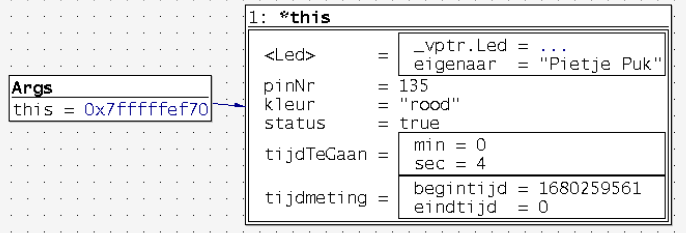
\includegraphics[width=0.95\textwidth]{figuren/ddd_logled_p2a}
				\caption{Logled met composities Tijdsduur en Stopwatch en associatie naar platform.}
				\label{fig:logObjectA}
			\end{subfigure}
			\begin{subfigure}[b]{0.49\textwidth}
				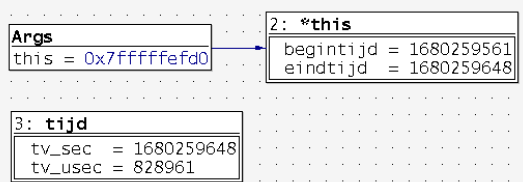
\includegraphics[width=0.95\textwidth]{figuren/ddd_logled_p2b}
				\caption{Van het object stopwatch, de attributen en lokale variabele tijd.}
				\label{fig:logObjectB}
			\end{subfigure}
			\caption{Inhoud van het object logled bij het aanroepen van de  zetUit() en vervolgens stap voor stap naar methode stop() van stopwatch.}
			\label{fig:logledOjecten}   
		\end{center}
	\end{figure}
 Bij figuur \ref{fig:logObjectB} zie je de waarde van de attributen van het object van de klasse \textit{Stopwatch} waarbij \textit{\textbf{tijd}} een lokale variabele is binnen de methoden \textit{void begin()} en \textit{void stop()} van de klasse Stopwatch.
\item Test kritisch en voer b.v. de test uit zoals in Listing \ref{lst:mainLogLed3} wordt weergegeven.
\begin{lstlisting}[caption= een tweede test om de logled uit te testen ,label={lst:mainLogLed3}]
int main (void)
{
	cout<<"hoi opgave2"<<endl;
	
	/* 
	De Rock pi wordt gebruikt om de pinnen aan te sturen.
	*/
	
	RockPi miniC(123456); //vul hier je eigen studienummer in.
	
	/*
	De Logled logld1 wordt aangesloten op pin18 en heeft
	als eigenaar Pietje Puk en een maximale brandtijd van 4 seconden.
	Bij logld2 is de eigenaar anoniem en heeft een maximale brandtijd van 2 seconden.
	*/ 
		
	Logled logld1(&miniC,18, "Rood", "Pietje Puk",4);
	Logled logld2(&miniC,23,2);
	
	cout<<"De eigenaar van ld1="<<logld1.deEigenaar()<<endl;
	cout<<"De eigenaar van ld1="<<logld2.deEigenaar()<<endl;
	
	logld1.zetAan();
	logld2.zetAan();
	usleep(TIMELEDON);
	logld1.zetUit();
	logld2.zetUit();
	usleep(TIMELEDOFF);
	logld1.zetAan();
	logld2.zetAan();
	usleep(TIMELEDON2);
	logld1.zetUit();
	logld2.zetUit();
	return 0 ;
}

\end{lstlisting}
\end{enumerate}

\end{comment}
